\documentclass[output=paper]{langscibook}
\ChapterDOI{10.5281/zenodo.10497373}

\author{Marta Rodríguez García \orcid{0000-0003-4104-0589} \affiliation{University of Basel}}
\title[The discursive construction of code-switching in Yanito]{The discursive construction of code-switching in Yanito among the young population of Gibraltar}

\abstract{Gibraltar is a small British enclave located in the south of the Iberian Peninsula. Despite its size, Gibraltar presents a historically, culturally, and linguistically rich landscape. Linguistically speaking, this speech community is characterised by a process of language shift in which Andalusian Spanish, the language of thousands of Gibraltarians before the 1970s, has slowly been replaced by the official language of the territory, British English. In this process, Yanito – a code-switching variety with lexicon from other Mediterranean languages – emerged as the vernacular language of the population. Despite the interest and complexity of this linguistic community, little is known about language variation or the use and evolution of this local dialect in younger speakers.

In this chapter, I study the structure and functionality of code-switching among young adults (16 to 35 years old) in Gibraltar in a sample of five focus groups collected between 2020 and 2021. I explore the use of code-switching in informal discourse from a more holistic perspective by combining structure and functionality. I first examine the fine line between structural categories and highlight categorical limitations between insertions and alternations. I then reflect on the importance of studying the functionality of code-switching from a sequential and interactional perspective. In doing so, this chapter offers a contribution to the literature on English and Spanish code-switching with an original methodology and from a European perspective. 
}


\IfFileExists{../localcommands.tex}{
   \addbibresource{../localbibliography.bib}
   % add all extra packages you need to load to this file

\usepackage{tabularx,multicol}
\usepackage{url}
\urlstyle{same}

\usepackage{listings}
\lstset{basicstyle=\ttfamily,tabsize=2,breaklines=true}

\usepackage{langsci-basic}
\usepackage{langsci-optional}
\usepackage{langsci-lgr}
\usepackage{langsci-osl}
% \usepackage{./langsci/styles/langsci-lgr}
% \usepackage{./langsci/styles/langsci-osl}
% \usepackage{langsci-gb4e}

\usepackage{tikz}
\usetikzlibrary{patterns,calc}
\pgfdeclarepatternformonly{south east lines}{\pgfqpoint{-0pt}{-0pt}}{\pgfqpoint{3pt}{3pt}}{\pgfqpoint{3pt}{3pt}}{
    \pgfsetlinewidth{0.6pt}
    \pgfpathmoveto{\pgfqpoint{0pt}{3pt}}
    \pgfpathlineto{\pgfqpoint{3pt}{0pt}}
    \pgfpathmoveto{\pgfqpoint{.2pt}{-.2pt}}
    \pgfpathlineto{\pgfqpoint{-.2pt}{.2pt}}
    \pgfpathmoveto{\pgfqpoint{3.2pt}{2.8pt}}
    \pgfpathlineto{\pgfqpoint{2.8pt}{3.2pt}}
    \pgfusepath{stroke}}
    
\usepackage{stmaryrd}
\usepackage{wasysym}
\usepackage{multirow}
\usepackage{caption}
\usepackage{subcaption}
\usepackage{mathrsfs}
\usepackage{qtree}

\usepackage{linguex}


   %pminos do not split footnotes
% \interfootnotelinepenalty=10000 %Footnote in Laporte chapters has to be split SN


%\DeclareIndexNameFormat{default}{%
%\nameparts{#1}%
%\usebibmacro{index:name}%
%{\index[names]}%
%{\namepartfamily}%
%{\namepartgiveni}%
% {}% L1
% {}% L2
%{\namepartprefix}% generates spurious space L3
%{\namepartsuffix}% generates spurious space L4
%}

%  {\DeclareIndexNameFormat{default}{%
%     \usebibmacro{index:name}{\index[names]}{#1}{#3}{#5}{#7}}}

%\DeclareIndexNameFormat{default}{%
%  \usebibmacro{index:name}{\sindex[nom]}{#1}{#3}{#5}{#7}}

%\DeclareIndexNameFormat{default}{%
%  \usebibmacro{index:name}{\sindex[person]}{#1}{#3}{#5}{#7}}
%\DeclareIndexNameFormat{default}{%
%\nameparts{#1} \usebibmacro{index:name}{\sindex[person]]}{\namepartfamily}{‌​\namepartgiven}{\nam‌​epartprefix}{\namepa‌​rtsuffix}}

%\newcommand{\smiley}{:)}

%\renewbibmacro*{index:name}[5]{%
%\usebibmacro{index:entry}{#1}%
%{\iffieldundef{usera}{}{\thefield{usera}\actualoperator}\mkbibindexname{#2}{#3}{#4}{#5}}}

% \newcommand{\noop}[1]{}

%remove for final
%\overfullrule=1mm

\newcommand{\tobi}[2]}}
\renewcommand{\S}[1]{\tobi{#1}{\textsc{*}}}

% this volume references
% puts: [this volume]
% already defined: \citetv
%\newcommand{\citepv}[1]{(\citeauthor{#1} \citeyear*{#1} [this volume])}
\newcommand{\citealtv}[1]{\citeauthor{#1} \citeyear*{#1} [this volume]}

%parentheses around example number
\newcommand{\pref}[1]{(\ref{#1})}

% in-text examples

\newcommand{\lnex}[1]{\textit{#1}} %target lang word
\newcommand{\lnlit}[1]{(lit.: `#1')} %literal reading
\newcommand{\lnlat}[1]{(#1)} % latinization
\newcommand{\lntrans}[1]{`#1'} %translation
\newcommand{\lnexl}[2]%
{\lnex{#1}{} \lnlat{#2}} % ex with latinization
\newcommand{\lnexlat}[3]{\lnex{#1}{} \lnlat{#2}{} \lntrans{#3}} % ex with latinization and tranl.

%ch01
\newcommand{\co}[1]{\mbox{\textbf{#1}}}

%ch09

\newcommand{\cyrbulg}[1]{\begin{otherlanguage*}{bulgarian}#1\end{otherlanguage*}}


%ch10
\newcommand{\nlp}{{\small NLP}}
\newcommand{\mwe}{{\small MWE}}
\newcommand{\rae}{{\small RAE}}
\newcommand{\lvc}{{\small LVC}}
\newcommand{\pos}{{\small P}o{\small S}}
%\newcommand{\todo}[1]{ \textcolor{red}{#1} }

%\renewcommand{\labelenumi}{\theenumi}
%\ainamefmt{{vv}{ll}{, ff}{, jj}} % fullname

\newcommand{\biberror}[1]{{\color{red}#1}}

\newcommand{\osenovaitem}{--~}
   %% hyphenation points for line breaks
%% Normally, automatic hyphenation in LaTeX is very good
%% If a word is mis-hyphenated, add it to this file
%%
%% add information to TeX file before \begin{document} with:
%% %% hyphenation points for line breaks
%% Normally, automatic hyphenation in LaTeX is very good
%% If a word is mis-hyphenated, add it to this file
%%
%% add information to TeX file before \begin{document} with:
%% %% hyphenation points for line breaks
%% Normally, automatic hyphenation in LaTeX is very good
%% If a word is mis-hyphenated, add it to this file
%%
%% add information to TeX file before \begin{document} with:
%% \include{localhyphenation}
\hyphenation{
    Beck-man
    Ngu-yen
    back-chan-nel
    back-chan-nels
    mo-not-o-nous
    ste-reo-typ-i-cal
}

\hyphenation{
    Beck-man
    Ngu-yen
    back-chan-nel
    back-chan-nels
    mo-not-o-nous
    ste-reo-typ-i-cal
}

\hyphenation{
    Beck-man
    Ngu-yen
    back-chan-nel
    back-chan-nels
    mo-not-o-nous
    ste-reo-typ-i-cal
}

   \boolfalse{bookcompile}
   \togglepaper[3]%%chapternumber
}{}


\begin{document}
\maketitle

\section{Introduction}\label{RG:sec:01}

Perched on the southern tip of the Iberian Peninsula, Gibraltar is one of the two Pillars of Hercules that marked the western limits of navigation for the ancient Mediterranean world. Consisting of a ridge rising 421 metres above sea level, the territory spans 6.8 square kilometres and is visible from the neighbouring areas in Spain and Africa. With a current population of around 34,000, Gibraltar has always been a melting pot of different cultures, languages, and religions. It has been a British overseas territory since 1713, at which point British English became its official language – coexisting with Andalusian Spanish, which kept being used as a lingua franca until language shift settled. This Spanish variety is also the language of the neighbouring community and is still spoken by some Gibraltarians in familiar and more informal settings (\citealt{moyer_analysis_1993}; \citealt{kellermann_new_2001}). 
The coexistence of these two languages, which differ in prestige and status, has resulted in a vernacular and code-switching variety known as \textit{Yanito}. Due to Gibraltar’s location and history, its community is not only bilingual, but in fact polyglot. The local linguistic repertoire and code-switching varieties are enriched with terms from Genoese, Hebrew, Arabic, Maltese, and Portuguese as a result of the human and commercial hustle and bustle that has characterised the history of the territory.


The border community of Gibraltar has been extensively studied and analysed by historians and anthropologists (\citealt{lopez_de_ayala_historia_1782}; \citealt{gold_gibraltar_2005}; \citealt{grocott_gibraltar_2012}). It has also captured the attention of linguists and sociolinguists 
(\citealt{lipski_sobre_1986}; \citealt{moyer_bilingual_1998}; \citeyear{moyer_pieter_2002}; \citealt{kellermann_new_2001}; \citealt{levey_language_2008}; \citealt{loureiro-porto_language_2017}; among others), who, over the course of time, have aimed to describe the social, cultural, and linguistic situation of this community. In particular, this study seeks to fill a gap in the literature on bilingualism and code-switching as a conversational strategy in the bilingual discourse of young adults in Gibraltar. It does so by taking a conversationalist and interactional approach to exploring the use of structural and functional categories that pose a challenge to the account of code-switching. Thereby, the analysis presented here adds to the comprehensive and growing literature on English–Spanish code-switching from the broader European context, which is of interest for comparative inquiries into bilingualism on a wider basis. The general purpose of this study is to explore (1) the structure of code-switching and (2) the function of code-switching in a sample of 15 speakers, distributed across five focus groups of young adults in Gibraltar aged between 16 and 35, and to stake out the field for further research on this topic.

\newpage
The chapter begins with a short description of the bilingual community of Gibraltar that reconstructs the social and historical processes that shape bilingualism and language shift (Section \ref{RG:sec:02}). The account of the methods that follows (Section \ref{RG:sec:03}) is unusually elaborate to allow for an informative description of the corpus generated by the five focus groups and a novel methodology, relying on a mystery game and the video-conferencing software Zoom. To achieve a more holistic picture of the complex phenomenon of code-switching in conversation, the analysis of the data combines two different angles: structural (Section \ref{RG:sec:04}) and functional (Section \ref{RG:sec:05}). Code-switching is first studied from a structural perspective, following Muysken’s strategies of code-switching (\citealt{muysken_bilingual_2000}; \citeyear{muysken_language_2013}), before being examined as a conversational and interactional tool by exploring language negotiation, turn-taking, and shifts in settings and topic.

\section{Language shift in Gibraltar}\label{RG:sec:02}

\subsection{From Spanish as a lingua franca to an English-only policy: Language shift in Gibraltar}
\label{RG:sec:02_1}

\begin{modquote}
Given what is happening in Gibraltar today, the way demographically Gibraltar is changing is concerning in some respects. For example, a lot of our young people are losing their second language, Spanish. We are losing bilingualism in favour of seeing a younger generation speak exclusively English. We want to control that if we can because bilingualism is an advantage. (Chief Minister Fabian Picardo, Uncorrected oral evidence: The UK-Spain agreement on Gibraltar 2021)
\end{modquote}

Despite major social and political changes, the linguistic situation in Gibraltar remained relatively stable until the 1970s
\citep{mariscal_rios_consecuencias_2014}. After the British conquest in 1713, English was introduced as the sole official language. However, Spanish, or more precisely, Andalusian Spanish, was still spoken by the vast majority of the population in a wide range of contexts and was even considered a lingua franca of the territory (\citealt{moyer_analysis_1993}; \citealt{mariscal_rios_consecuencias_2014}). After the Second World War, several factors contributed to major changes in the linguistic situation in Gibraltar and the establishment of an English-only policy. These included the evacuation of the civil population to other British territories and the return to Gibraltar of those families after the war, the introduction of the British schooling system, the closure of the border with Spain between 1969 and 1981, and the development of negative attitudes towards Spain and the Spanish language that promoted the use of English and the concept of English as ‘the language of opportunities’. From the 1970s onwards, British English has been increasingly established as a significant part of the linguistic landscape, along with Gibraltarian English
(\citealt{levey_schreier_gibraltar_2015}; \citealt{suarez-gomez_english_2020}), and a diminished Andalusian Spanish.

%%%%
%%%%\begin{figure}[h] %TODO: Grafik einfügen
%%%%  \includegraphics[width=0.8\textwidth]{RG_Figure_1.png}
%%%%  \caption{Language shift in Gibraltar from diglossia to diaglossia/dilalia \citep{rodriguez_garcia_role_2021}}
%%%%  \label{RG:fig:1n}
%%%%\end{figure}


\begin{figure}[h]

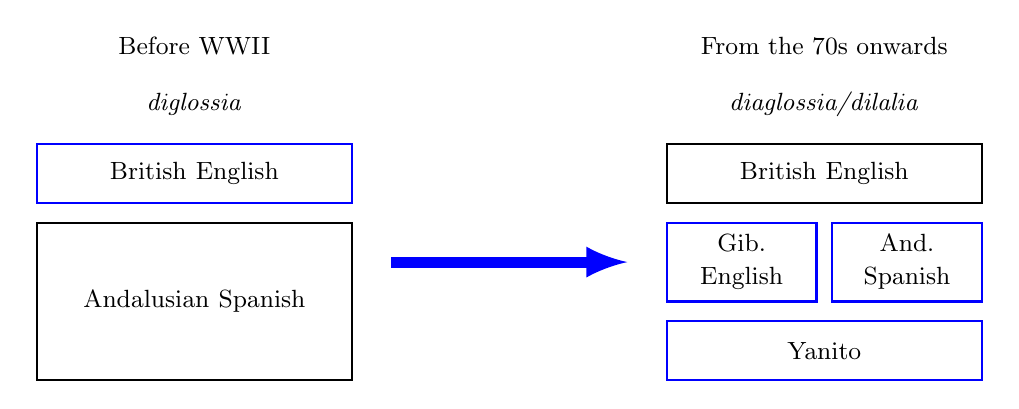
\begin{tikzpicture}

\node at (2,1.25)[align=center] {\small Before WWII};
\node at (2,.5)[align=center] {\small \textit{diglossia}};


\node at (10,1.25)[align=center] {\small From the 70s onwards};
\node at (10,.5)[align=center] {\small \textit{diaglossia/dilalia}};


\draw[color=blue, thick](0,0) rectangle (4,-.75) node[color=black, pos=0.5, text width=4cm,align=center] {\small British English};
\draw[thick](0,-1) rectangle (4,-3) node[pos=0.5, text width=4cm,align=center] {\small  Andalusian Spanish};

\draw[-latex,blue,line width=4pt] (4.5,-1.5)--(7.5,-1.5);

\draw[thick](8,0) rectangle (12,-.75) node[pos=0.5, text width=4cm,align=center] {\small  British English};

\draw[color=blue, thick](8,-1) rectangle (9.9,-2) node[color=black, pos=0.5, text width=1.6cm,align=center] {\small  Gib. English};
\draw[color=blue, thick](10.1,-1) rectangle (12,-2) node[color=black, pos=0.5, text width=1.6cm,align=center] {\small  And. Spanish};

\draw[color=blue, thick] (8,-2.25) rectangle (12,-3) node[color=black, pos=0.5, text width=4cm,align=center] {\small  Yanito};
 

\end{tikzpicture}

  \caption{Language shift in Gibraltar from diglossia to diaglossia/dilalia \citep{rodriguez_garcia_role_2021}.}
  \label{RG:fig:1}
\end{figure}


\autoref{RG:fig:1} shows that the territory has undergone significant linguistic changes. From an extended diglossia
(\citealt{fishman_bilingualism_1967}; \citealt{auer_postscript_2005})  with British English as the ‘high variety’ and Andalusian Spanish as the ‘low variety’, there has been a development to what could be better described as diaglossia \citep{auer_postscript_2005} or dilalia \citep{berruto_hinskens_dialectstandard_2005}. This means that the structural and functional separation between the standard language and the local varieties, as well as the domains and specific pragmatic functions for each language, can no longer be clearly drawn. The bilingual situation is marked by intermediate variants between standard and dialect varieties and speakers shifting from a dialectal variant to a standard one, adapting to their situation and their audience \citep{rodriguez_garcia_role_2021}. Shifts can be encouraged by several factors and situations, such as the relationship between speakers and the formality of the speech events, the topic of the conversation, and the medium (\citealt{auer_postscript_2005}; \citeyear{auer_language_2014}). This is where Yanito, as the local code-switching variety, emerges. 

Local writers and former educators such as Charles Durante believe there is a need to raise awareness of Gibraltar’s linguistic richness \citep{durante_charles_2019} and value Yanito as a local form of communication that fosters social interaction, creates a sense of belonging, and reinforces the identity of the Gibraltarian, thereby allowing people to be identified both within and outside their community. However, as an oral and local variety, Yanito is exposed to constant variation across generations. This article examines the current variant of Yanito used by a new generation of young adults and highlights code-switching patterns observed in a small sample of young adult speakers.

\subsection{	Code-switching in Gibraltar }
\label{RG:sec:02_2}

Code-switching is a widely used strategy to enhance linguistic and social identity in bilingual and multilingual contexts; it is also a gauge of sociolinguistic processes and changes in such communities. In this context, Gibraltar presents a complex sociolinguistic situation in which Yanito – which I define here as the local speech variety characterised mainly by English–Spanish code-switching – is widespread and enjoys certain covert prestige among speakers. However, the current language shift is affecting Yanito. The decline in popularity of Spanish among younger Gibraltarians, resulting from the introduction of English as a medium of instruction in school after the Second World War, and the dominance of English in private and public spheres are reshaping communication and the distribution of languages in conversation. 

Code-switching eludes easy explanation, as recognised by experts like \citet{myers-scotton_review_2002},
\citet{gumperz_sociolinguistic_1977}, and 
\citet{auer_code-switching_1998}, who have all long tried to account for the multiple factors affecting and conditioning the choice of a code in conversations, discourses, and interactions. This general difficulty is exacerbated by the well-documented differences in various bilingual communities. Hence, for the purpose of this chapter, I combine Auer’s (\citeyear{auer_code-switching_1998}) and Gumperz’s (\citeyear{gumperz_sociolinguistic_1977}) broad definitions of the term, which have served as suitable definitions for numerous studies on code-switching over the decades due to their flexibility and adaptability. Based on both authors, I understand code-switching as “the juxtaposition of passages of speech belonging to (at least) two different grammatical and semiotic systems, within the same exchange” \citep[1]{gumperz_sociolinguistic_1977}. This broad definition makes it possible to adopt a functional and holistic approach to the phenomenon of code-switching. This facilitates a nuanced understanding of the function and sequential organisation of code-switching in conversation and explains bilingual conversation in relation to language choices at a conversational and interactional level. 

Existing research on the linguistic situation of Gibraltar points towards the generational loss of Spanish and to language shift
(\citealt{moyer_analysis_1993}; \citealt{kellermann_new_2001}; \citealt{feijoo_rodriguez_somos_2015})
and focuses on the local code-switching variety and its form – accounting for both its use in familiar and informal situations and the complexity of its form and function. The twentieth century witnessed an increasing interest in the structures of bilingual speech in Gibraltar, and although much of this interest is confined to unpublished master’s theses, there are several investigations and ongoing projects pointing to rich and variable code-switching strategies in Gibraltar. These strategies include the selection of a main language for interaction, the negotiation of languages between turns, and various examples of intersentential and intrasentential code-switching behaviour \citep{moyer_bilingual_1998}. More recent studies on Yanito shed light on the reduction in the use and variety of bilingual structures. For instance, \citet{goria_functional_2017} reports the rise of a mixed code involving the use of fixed switching patterns in which the direction of the switch is constrained and the pragmatic meaning behind the use of certain bilingual markers is lost. Furthermore, \citet{weston_code-switching_2013}  offers evidence of notable diachronic and synchronic differences at the individual level, demonstrating the need for further research at both individual and community level. 

Although methods used to study Yanito have become more systematic, the corpora still lack sufficient data on younger generations of speakers. This data gap makes it difficult to provide an account of the current state of bilingual discourse in younger Gibraltarian generations. While the loss of Spanish in favour of English is undeniable at a community level, more has to be done to understand the state of Yanito. A preliminary study by
\citet{chevasco_contemporary_2019} on language use and attitudes registers an unexpected increase in the use of and positive attitudes towards Yanito among young adults in informal and family settings, and reports Yanito as an important symbol of identity and as a strategy to reaffirm local identity in relaxed conversations \citep[63]{chevasco_contemporary_2019}. 

An in-depth study of code-switching in younger generations which accounts for both structure and functionality promises a substantiated understanding of the linguistic situation of this territory and the future of code-switching in that setting. Based on the well-established knowledge that bilingual speech may be influenced by a great number of external factors (e.g., the communicative situation, the participants, the topic, etc.) and internal factors (e.g., grammatical constraints, the languages involved, the proficiency of speakers, etc.), I study the bilingual speech of young adults in Gibraltar as a communicative strategy with social meaning.

\section{Methodology and research corpus}\label{RG:sec:03}

Previous literature has found that Yanito often appears in informal local conversations and that it can be triggered by various factors, such as the relationship between participants and the topic and purpose of the conversation (\citealt{moyer_analysis_1993}; \citealt{kellermann_new_2001}; \citealt{levey_language_2008}; \citealt{weston_code-switching_2013}). Therefore, a flexible methodology which can account for the different situations that trigger code-switching is needed. A pilot study in which I conducted semi-directed interviews confirmed the value of focus groups, where participants discuss various topics with people who are close to them, such as friends or family members, following guidelines for the conversation that contain topics, pictures, statements, and a game. The use of the (online) focus-group technique, as well as the guidelines with topics and activities for the conversation and the close relationship between participants, made it possible to observe language in a nearly natural manner while covering topics of interest for the study \citep{labov_field_1984}. The guidelines comprise three parts. The first prompts participants to converse about various topics, from informal subjects (childhood memories, funny anecdotes, and holidays) to more formal topics (e.g., COVID-19 and political measures, education, job opportunities). In part two, participants are given visual and written prompts that encourage them to converse about the influence of different cultural, linguistic, and identity-related aspects. The pictures depict cultural festivities and items and images of the border, the late Queen Elizabeth II, or the Prime Minister of Gibraltar. The written statements are from Gibraltarians and refer to the local code-switching variety and the multiculturality of the territory. Here, again, the formality of the topic changes according to the pictures and the situations the participants describe. Emotions such as nostalgia, happiness, or anger appear often and impact the participants’ language. Finally, in part three, participants play a mystery game in which they have to solve a case by reading and talking about a series of bilingual cues. This part makes it possible to observe the language participants use while playing and how they react to Spanish input. Overall, the focus groups enabled me to gather data that allow a close analysis of code-switching and its functionality; namely, the well-known characterisations of situational, metaphorical, and conversational switching. After finishing this conversation, participants are asked to complete an online questionnaire that collects socio-demographic information and individual participants’ views on language use and competence. Given the constraints on fieldwork during the COVID-19 pandemic, I opted for an online, corpus-based methodology with focus groups of three people each. As it was difficult to recruit younger participants (aged between 16 and 21), the online corpus was supplemented with data gathered in face-to-face interactions in May 2021 in three state secondary schools – Westside School, Bayside School, and Gibraltar College – following the same focus-group methodology.

The groups were established on the basis of age in order to determine how the language shift process is reflected in the language of young adults. The age groups were created attending to historical and social criteria. Concretely, the first age group (A) corresponds to school students with little experience abroad who were born in the 2000s (therefore, born and raised in a European and open-border Gibraltar); group (B) corresponds to young adults who were born during the launch of the European Economic Union and with possible experience abroad (educational or professional purposes); and group (C) represents those who were born in a period of memories and resentment and a less porous border, but who also experienced a more balanced bilingualism within the community (those may also be the parents of a new generation). As it can be seen, the division of the groups according to age allows to explore language behaviour as a reflection of political, historical, social, and linguistic changes.


\begin{table}[h]
  \begin{tabularx}{\textwidth}{XXXl}\midrule\toprule
Age group A &Age group B 	&
Age group C 	&Mixed group\\ 
(16 to 21)	&(22 to 28) &(29 to 35)\\
\midrule
A1 &	B1 &	C1&	BA1\\
&	B2 		\\
 \bottomrule\midrule
  \end{tabularx}  \caption{Distribution of five focus groups (sample for analysis).}
  \label{RG:tab:1}
\end{table}


For this chapter, a first sample of five focus groups was studied (see \autoref{RG:tab:1}): one focus group of younger speakers aged between 16 and 21 (A1); two focus groups of speakers aged between 22 and 28 (B1 and B2); one focus group of older speakers aged between 29 and 35 (C1); and one mixed group with speakers in the younger or middle age ranges (BA1). The sample was balanced, albeit small, totalling 15 participants. It included people with diverse cultural, ethnic, and religious backgrounds who had had diverse experiences abroad. In fact, 9 out of the 15 participants of this study confirmed having educational or professional experiences abroad. A gender balance was also achieved. The focus group discussions lasted approximately 30 to 45 minutes each. For the analysis, a total of 241 minutes (approximately 40,800 words) of interaction was transcribed in ELAN and subsequently analysed. In this first exploratory analysis, I used orthographic transcription to account for cases of code-switching, then classified the occurrences attending to the structural patterns. This was followed by a qualitative analysis of the instances with a focus on the sequence of the conversation and the structure of the discourse in order to explore the functions of code-switches. The results obtained from this provided a basis for determining which avenues of inquiry would be most promising for further research.

The examples provided for the analysis (Section \ref{RG:sec:04} and \ref{RG:sec:05}) are extracted from the original transcriptions and followed by the English translation. For a better understanding of the examples, an appendix with transcription conventions is attached at the end of the chapter. 

\section{Yanito from a structural perspective}\label{RG:sec:04}

For the structural analysis, I focus on three patterns proposed by \citet{muysken_language_2013}: insertion, alternation, and backflagging. The first structural pattern, insertion, refers to a chunk of language B – in this case, Spanish – inserted into a sentence in language A – in this case, English \citep[712]{muysken_language_2013}.

\begin{exe}\ex\label{RG:ex1}
SOPHIA: \footnote{In order to maintain the anonymity of the participants, a code was attributed to them. The names that appear in this chapter are fictitious, but they have been selected from names heard in Gibraltar during my research stays.} 
 \textit{La querida} (.) why should why should \textit{la querida} want to: maybe he’s maybe he was gonna leave his wife \textit{para la querida}\\
SOPHIA: \ul{The lover} (.) why should why should \ul{the lover} want to: maybe he was gonna leave his wife \ul{for the lover}
\end{exe}


In Example (\ref{RG:ex1}), the lexical element \textit{querida}, meaning ‘mistress’, appears together with the feminine definite article \textit{la} inserted into an English clause. The expression \textit{la querida} is taken from Spanish without affecting the structure of the sentence. In examples of insertion, we observe that single elements of language B are inserted within an otherwise language A clause. Sometimes, however, we find that a longer chunk of text of language B, which constitutes a clause, alternates with a chunk of text in language A, as in the following example from Sophia, a speaker from group C1.

\begin{exe}\ex\label{RG:ex2}
SOPHIA: \textit{Vamos a ver dónde está esto} | can you send me a screenshot?\\
SOPHIA: \ul{Let’s see where this is} | can you send me a screenshot?
\end{exe}

Example (\ref{RG:ex2}) is a clear case of alternation or “a succession of fragments in language A and B in a sentence” \citep[713]{muysken_language_2013}. In this case, there is a first declarative statement in Spanish which is followed by a question in English. The appearance of a Spanish utterance at the left margin of a new context is very common among speakers from different focus groups. However, this phenomenon is not consistent among speakers, and alternations appear as a result of participant- and discourse-related switches, especially in language negotiation. 

This leads to the next pattern: backflagging. According to \citet[713]{muysken_language_2013}, in this structural pattern, discourse markers from a heritage language are inserted in a sentence in an L2. This is the most common and consistent pattern among young adult speakers in Gibraltar. However, it is worth noting that the matrix language of the sentence, English, constitutes the L1 or language A for most of the speakers in my corpus. In the speech of young Gibraltarian adults, the insertion of Spanish markers into an otherwise English discourse is noteworthy \citep{goria_functional_2017}, even if they do not consider themselves intermediate or advanced speakers of Spanish, as stated in my socio-demographic and linguistic questionnaire and sometimes in the focus group itself. In this way, the markers could be some kind of ‘inherited’ material from previous generations or even a symbol of identity for younger generations. It is common among the five groups to find examples of the use of discourse markers such as \textit{pero} and \textit{bueno} or the question tag \textit{¿no?} On many occasions, they appear as single insertions within an otherwise English clause. In Example (\ref{RG:ex3}), Sophia makes use of the discourse marker \textit{bueno} to take her turn, change the topic of the conversation, and initiate the clause.

\begin{exe}\ex\label{RG:ex3}
SOPHIA: \textit{Bueno} should we think of like anecdotes or funny moments?

SOPHIA: \ul{Well} should we think of like anecdotes or funny moments?
\end{exe}

All three types of structural strategies described by Muysken are found in the corpus. In some cases, the three types appear in the discourse of the same speaker, as has been illustrated in the case of Sophia in Examples (\ref{RG:ex1}), (\ref{RG:ex2}) and (\ref{RG:ex3}), while in some groups, certain patterns are more consistent in one speaker than others. \autoref{RG:tab:2} outlines the phenomena found in the analysis of the five focus groups.


\begin{table}[h]
  \begin{tabularx}{\textwidth}{lccccc}\midrule\toprule
Code-switching strategies &	A1&	B1	&B2	&BA1	& C1\\ \midrule
Insertion &Sp > E	&*Sp > E &	Sp > E 	&Sp > E	&*Sp > E   \\
Alternation  &(\surd) &\surd &(\surd) &(\surd) &\surd\\
Backflagging   &\surd &\surd &\surd &\surd &\surd \\
 \bottomrule\midrule
  \end{tabularx}  \caption{Structural patterns found in the focus groups.}
  \label{RG:tab:2}
\end{table}

As illustrated in \autoref{RG:tab:2}, all patterns emerge in the five focus groups. However, insertion is the most common pattern among speakers, together with backflagging, which is also the most consistent one. In the case of insertion, I find both English and Spanish insertions in groups B1 and C1. The directionality of the switch is not always clear and this is why those groups are marked with an asterisk in the table. This is something worth studying, since previous studies on Gibraltar account for the insertion of elements from a dominant and prestigious language into a less prestigious or non-dominant language, but not in the opposite direction – something that is also very common in my corpus (\citealt{moyer_bilingual_1998}; \citealt{feijoo_rodriguez_somos_2015}). In the case of alternations, greater differences among speakers in the same conversation can be observed, and while age seems to play a role in the use of different patterns of alternations and insertions, this is clearly not the only factor. In some cases, speakers who belong to the same age group show great variation in the use of alternation, such as in A1, B2, and the mixed group, BA1. In the process of classifying the examples from the corpus, the distinction between insertions and alternations occasionally becomes fuzzy. Speakers make use of longer insertions such as \textit{y todo ese rollo} ‘and all that stuff’ which are difficult to classify according to structural parameters, as illustrated in Example (\ref{RG:ex4}). The Spanish sentence starts with the conjunction \textit{y} ‘and’, followed by the indefinite pronoun \textit{todo} ‘all’ and the demonstrative \textit{ese} ‘that’, which precede the noun \textit{rollo}, in this case, ‘stuff’. This cluster serves as a way of closing the previous topic but also serves to start the next alternation. In this case, Spanish is identifiable as language B in the quote, but the chunk results in a bigger switch to language B.

\begin{exe}\ex\label{RG:ex4}
MOHAMED:  The university (.) what have affected you guys? Tell us more about \textit{bueno} you mentioned \textit{que} they’ve contacted you for eh test when you go back home for Christmas \textit{y todo ese rollo} so \textit{es un rollo pero al mismo tiempo} | it’s maybe a mess \textit{¿no?}\\

MOHAMED: The university (.) what have affected you guys? Tell us more about \ul{well} you mentioned \ul{that} they’ve contacted you for eh test when you go back home for Christmas \ul{and all that stuff} so \ul{it’s (messy) stuff but at the same time} | it’s maybe a mess \ul{isn’t it?}
\end{exe}

The functionality of the chunk \textit{y todo ese rollo} in language B, Spanish, is also similar to structural markers or discourse organisers, since it serves as a recurrent mechanism for the speaker to close a topic. But later, the same noun \textit{rollo} serves different purposes in the subsequent alternation. As I mentioned, the insertion of discourse markers is very common among young adult speakers. The examples observed again raise the question of whether they should be considered code-switching, as their form is similar to insertion. However, the use of more complex discourse markers and the combination of elements stress the need to pay special attention to the use of these pragmatic, discursive elements.

\largerpage
\begin{exe}\ex\label{RG:ex5}
MOHAMED:  Our identity rests solely on on on being part of [Britain \textit{ahí está ahí está} on being part of Britain]\\
AKRAM: [our history yeah the history of Gibraltar \textit{sí señor}]\\
MOHAMED: \textit{escúchame el nuevo} Bayside \textit{García y los colegas}\\
AKRAM: social distancing social distancing\\
MOHAMED: \textit{es que} none of us none of us were able to actually to enjoy the new Bayside \textit{esa es la cosa}\\

MOHAMED: Our identity rests solely on on on being part of [Britain \ul{there you are there you are} on being part of Britain]\\
AKRAM: [our history yeah the history of Gibraltar \ul{yes, sir}]\\
MOHAMED: \ul{listen to me the new} Bayside \ul{García and the friends}\\
AKRAM: social distancing social distancing\\
MOHAMED: \ul{that is} none of us none of us were able to actually to enjoy the new Bayside \ul{that’s the thing}
\end{exe}

In this short extract from a conversation between two young males in Example (\ref{RG:ex5}), different markers enter into play: to express agreement, such as \textit{ahí está} ‘there you are’ or \textit{sí señor} ‘yes, sir’; to get attention and initiate a new topic, such as \textit{escúchame} ‘listen to me’; and to initiate and close an intervention, such as \textit{es que} ‘is that’ and \textit{esa es la cosa} ‘that’s the thing’. As observed, their form and functionality are also of a different complexity, which makes it difficult to label them or group them into categories. Further research has to be done to study the functionality of those markers and to observe if their meaning and use comes from Spanish or English, or even if new meanings are arising from the contact of both languages. This question leads us to the same previous dichotomy of insertions versus alternations and even to code-switching versus code-mixing \citep{auer_code-switching_1998}. The complexity of the markers is higher among older speakers, as illustrated in an extract between two participants from group C1 in Example (\ref{RG:ex6}). Here, the combination of markers is very common among different participants (more than 100 instances of combinations of Spanish markers and around 70 combinations of Spanish and English markers), as in the example of \textit{bueno espérate ¿te acuerdas?} ‘well, wait, do you remember?’.

\begin{exe}\ex\label{RG:ex6}
LAURA:  And it was dark on the way back and you were thinking if I run over a car (.) \textit{no pasa nada} you have to run it over \textit{¿te acuerdas?}\\
HELEN: yes (4.1) \textit{bueno espérate ¿te acuerdas?} Was this the same time on the way back?\\
LAURA: ye::s that was pitch bla::ck!\\

LAURA: And it was dark on the way back and you were thinking if I run over a car (.) \ul{nothing happens} you have to run it over \ul{do you remember?}\\
HELEN: yes (4.1) \ul{well wait do you remember?} Was this the same time on the way back?\\
LAURA: ye::s that was pitch bla::ck!
\end{exe}

The function of the whole phrase \textit{bueno espérate} is reminiscent of an utterance employed by Sophia – from the same focus group C1 – at another point in the conversation in which she makes use of the element \textit{un momentito}, ‘a moment’ (Sophia: I’m just gonna quickly have a look at the questions \textit{vale un momentito}? (.) I’m just gonna put […]). In the case of \textit{bueno espérate}, the chunk serves as strategy to give the speaker time to think about something and to do something in the case of \textit{un momentito}, that is immediately followed by a stop. In particular, the use of discourse markers from the heritage language, Spanish, seems to show characteristics from both insertions and alternations, making it difficult to define the code-switching patterns. Sentential based classifications, such as Poplack’s (\citeyear{poplack_sometimes_1980}) inter- and intrasentential switching could help solving some of these difficulties, but it still seems clear that there is a strong need to further study the functionality of groups of structural patterns within discourse in order to account for the use of both languages in Gibraltar. 

By analysing the structure of code-switching, we can better visualise the factors, strategies, and outcomes in code-switching. In addition, it also helps to justify language shift within a community by studying the matrix language and the directionality of the switch; English is by far the preferred language and the matrix language in most cases, while switches to Spanish appear often, whereas previous studies on first and second generations have shown completely the opposite distribution of languages (\citealt{moyer_analysis_1993}; \citealt{kellermann_new_2001}; \citealt{weston_code-switching_2013}). Something I also observed in the examples is the peripheral location of the switches to Spanish, which tend to appear to the left (in most cases) or to the right of the turn (ongoing analysis, see \cite{goria_complex_2021}). However, it seems that structure is not enough to understand how speakers code-switch and why they do it. Therefore, a detailed study of the functionality of those patterns in conversations and interactions is needed in order to better understand the motivation of the speakers, which I will turn to in the next section.

\section{Yanito from a discursive and conversational perspective}\label{RG:sec:05}

\subsection{Language negotiation}\label{RG:sec:05_1}
\largerpage
When initiating a conversation or when there is a change in a setting or in terms of the participants, speakers adapt their speech to the new environment. In this section, I present some examples that account for the alignment of participants in interaction and the distribution of languages by turns. In some cases, the three participants of the focus group change the code from the beginning of the conversation and show a rich repertoire of bilingual structural strategies, as in the case of C1 in Example (\ref{RG:ex7}).\clearpage

\begin{exe}\ex\label{RG:ex7}
SOPHIA:  Girls\\
HELEN: [okay]\\
SOPHIA: [(…)]\\
HELEN: okay \textit{bueno} [let’s start]\\
SOPHIA: [I don’t wanna touch] my phone and I’ve got the questions \textit{mira en el} laptop\\
LAURA: \textit{y yo y yo} my [laptop is (…)]\\
HELEN: \textit{bueno} [let’s (.) \textit{¿qué dice?}]\\
LAURA: we met in school!\\
HELEN: \textit{bueno espérate} let’s go through the first section ((reading the guideline)) “your friendship (.) how did everything start?”\\
LAURA: I don’t know\\
SOPHIA: Westside \textit{¿no?} I think it started\\
LAURA: we were all in different schools \textit{¿no?}\\
HELEN: \textit{sí yo} [\textit{fui a:}] \\
SOPHIA: yeah Westside\\
HELEN: \textit{yo fui a} Saint Catherine’s first school \textit{y después} Sacred Heart\\

SOPHIA: Girls\\
HELEN: [okay]\\
SOPHIA: [(…)]\\
HELEN: okay \ul{well} [let’s start]\\
SOPHIA: [I don’t wanna touch] my phone and I’ve got the questions \ul{look on the} laptop\\
LAURA: \ul{and I and I} my [laptop is (…)]\\
HELEN: \ul{well} [let’s (.) \ul{what do you say?}]\\
LAURA: we met in school\\
HELEN: \ul{well wait} let’s go through the first section ((reading the guideline)) “your friendship (.) how did everything start?”\\
LAURA: I don’t know\\
SOPHIA: Westside \ul{wasn’t it}? I think it started\\
LAURA: we were all in different schools \ul{weren’t we?}\\
HELEN: \ul{yes I [I went to]}\\
SOPHIA: yeah Westside\\
HELEN: \ul{I went to} Saint Catherine’s first school \ul{and then} Sacred Heart
\end{exe}

In Example (\ref{RG:ex7}), the speakers start the conversation by establishing English as their matrix language, but Helen quickly starts inserting Spanish elements, such as the marker \textit{bueno} ‘well’ to get the attention of the other speakers, to which Sophia reacts with a bigger switch: an alternation with an English insertion (\textit{mira en el laptop} ‘look on the laptop’) at the end of her intervention, accepting the switch as a strategy for the conversation. Laura also initiates her turn in Spanish (\textit{y yo y yo} ‘and me and me’) as a response of agreement to the use of both languages in interaction. In this example of language negotiation, we observe that even though English is used as the language of communication, speakers agree on using Spanish for participant-related purposes, such as agreeing on ideas – \textit{y yo y yo} ‘and me and me’ and \textit{sí} ‘yes’ – or reacting to a previous interaction – \textit{¿qué dice?} ‘what do you say’ and \textit{espérate} ‘wait’. Spanish is also used for discursive purposes by framing the sequentiality of the events, for example with \textit{y después} ‘and then’. Speakers agree on the language of interaction because they all know that their proficiency and linguistic strategies are similar, which also makes speakers display a great number of structural strategies of code-switching within the conversation. This is more an exception than the norm, since in most of the focus groups, speakers take longer to negotiate the language of communication.

In the B1 group, two speakers with a high level of proficiency in both languages (Daniel and David) switch from English to Spanish on multiple occasions, while Alex uses English most of the time, as can be seen in Example (\ref{RG:ex8}).

\begin{exe}\ex\label{RG:ex8}
ALEX:  We used to be in different schools and in different football teams and then we played together (.) for the selection (.) for the gfa\\
DANIEL: ((addressing David)) \textit{¿te acuerdas que jugabas con él o no? ¿y era bueno de chico?}\\
DAVID: \textit{malísimo} (.) \textit{bueno} ((addressing Alex)) recently \textit{te di la foto::}\\
ALEX: yeah recently you gave me (.) actually\\
DANIEL: \textit{¿y eso qué era} gfa? \\
DAVID: \textit{Entonces (año) nueve}\\
DANIEL: (under the) eleven rather than\\
DAVID: and eh:: eleven \textit{sería ¿no?} or on the ninth ((addressing Alex))\\
ALEX: or the ninth ninth (.) we were younger\\
DAVID: yeah\\
ALEX: ((addressing Daniel)) \textit{¿y tú?}\\
DANIEL: me what?\\
ALEX: knowing David\\
DANIEL: David? (0.7) \textit{¿de dónde nos conocemos?} ((addressing David)) \textit{ahí en la escuela ¿no?}\\

ALEX: We used to be in different schools and in different football teams and then we played together (.) for the selection (.) for the gfa\\
DANIEL: ((addressing David)) \ul{do you remember that you played with him or not? And was he good as a child?}\\
DAVID: \ul{very bad (.) well} ((addressing Alex)) recently \ul{I gave you the picture}\\
ALEX: yeah recently you gave me (.) actually\\
DANIEL: \ul{and what was that} gfa?\\
DAVID: \ul{then (year) nine}\\
DANIEL: (under the) eleven rather than\\
DAVID: and eh:: eleven \ul{would be wouldn’t it?} Or the ninth ((addressing Alex))\\
ALEX: or the ninth ninth (.) we were younger\\
DAVID: yeah\\
ALEX: ((addressing Daniel)) \ul{and you?}\\
DANIEL: me what?\\
ALEX: knowing David\\
DANIEL: David? (0.7) \ul{from where do we know each other?} ((addressing David)) \ul{there in the school wasn’t it?}
\end{exe}

Speakers switch and accommodate in many parts of this conversation when addressing each other. In Example (\ref{RG:ex8}), Alex accommodates Daniel by using Spanish when asking him how he met David with the question \textit{¿y tú?}, ‘and you?’; Daniel responds in English, accommodating Alex’s language preference (me what?) and switches again to Spanish when he looks for confirmation from David as to where they got to know each other (\textit{¿de dónde nos conocemos?}). In the case of B1, the group seems to be very aware of their linguistic preferences, even though they are probably not aware of their multiple accommodations during the conversation and the increase in the use of Spanish in Alex’s interventions. They even mention this explicitly when discussing language shift and the linguistic situation of Gibraltar (see Example \ref{RG:ex9}).

\begin{exe}\ex\label{RG:ex9}
ALEX:  \textit{No} we mix a lot \textit{sin darnos cuenta, la verdad}\\
DANIEL: \textit{pero lo bueno es que los padres hablan español y los niños} [\textit{no hablan ¿cómo puede ser?}]\\
DAVID: [\textit{y los niños no (no hablan) mi her}[\textit{mano}]\\
ALEX: [\textit{mi hermana}] (.) \textit{mi hermana igual}\\
DANIEL: ((addressing David)) \textit{bueno tú hablas mucho más español que tu hermano}\\
DAVID: \textit{mi hermano no lo habla pero todos los amigos de mi hermano son ingleses de Soto (.) esos son tan} English \\
DANIEL: \textit{pero lo sabe}\\
ALEX: yeah I know\\
DANIEL: \textit{pero ¿los padres tuyos?}\\
ALEX: it’s more English yeah\\
DANIEL: ah they don’t speak Spanish\\
DAVID: they don’t speak \textit{así}\\
ALEX: \textit{mi hermana no habla nada eh}\\
DANIEL: \textit{claro le cuesta (.) tú ahora hablas mucho más que antes} (.) probably because of us\\
ALEX: probably\\

ALEX: \ul{Not} we mix a lot \ul{without realising, that’s the truth}\\
DANIEL: \ul{but well the thing is that the parents speak Spanish and the children [don’t speak how can it be?]}\\
DAVID: \ul{[and the children don’t (don’t speak) my brother]}\\
ALEX: \ul{[my sister] (.) my sister is the same}\\
DANIEL: ((addressing David)) \ul{well you speak much more Spanish than your brother}\\
DAVID: \ul{my brother doesn’t speak it but all the friends of my brother are English from Soto (.) those are so} English\\
DANIEL: \ul{but he can/knows}\\
ALEX: yeah I know\\
DANIEL: \ul{but your parents?}\\
ALEX: it’s more English yeah\\
DANIEL: \ul{ah} they don’t speak Spanish\\
DAVID: they don’t speak \ul{like that}\\
ALEX: \ul{my sister doesn’t speak at all}\\
DANIEL: \ul{of course it’s hard for her (.) you speak now much more than before} (.) probably because of us\\
ALEX: probably
\end{exe}

In Example (\ref{RG:ex9}), the speakers discuss the loss of Spanish in younger generations, starting with the following statement: ‘Parents speak Spanish and their children don’t’ but they also reflect on their own situation and their linguistic preferences. They discuss the fact that their siblings are also speaking less Spanish because of their English friends and that Alex speaks Spanish even though his parents speak more English at home. Here, Daniel concludes that the fact that Alex has improved his level and use of Spanish may be \textit{because of us}. This could refer to their current friendship, but probably also to the fact that they teach in the same school, which makes them spend a lot of time together.

Even though younger generations make more use of English, as the three speakers from the B1 group state, I still observed differences between participants in group A1. While most of them prefer to use English almost exclusively, others make use of both languages in discourse and even force English speakers to accommodate. In Example (10), the three speakers aged 17 and 18 discuss their holidays in Spain. In this part of the conversation, it seems that Dan wants Mike to switch to Spanish since he keeps asking him in this language (‘where do you go’, ‘where in Spain?’, ‘with your family?’, ‘your friends as well or not?’) and only stops asking for more information when Mike finally replies in Spanish: \textit{sí hermano} ‘yes, brother’ and \textit{no}.

\begin{exe}\ex\label{RG:ex10}
MIKE:  I didn’t go on holiday last year ‘cause Covid same as Lyan (.) and (.) I’ll be going on holidays this year in July middle of July\\
LYAN: \textit{¿qué más? ¿adónde }[\textit{vas?}]\\
DAN: [\textit{dónde vas}]\\
MIKE: Spain\\
LYAN:\textit{ pero ¿a dónde en España?}\\
DAN: \textit{Estepona::}\\
MIKE: yes \textit{Estepona}\\
LYAN: with a pool (.) bar?\\
MIKE: a villa\\
DAN: \textit{ah vale con tu familia ¿no?}\\
MIKE: \textit{sí hermano}\\
DAN: \textit{¿tus amigos también o no?}\\
MIKE: \textit{no}\\
DAN: (0.7) \textit{ah vale} (.) \textit{perfecto}\\
LYAN: \textit{vale está bien ahora vamos hablar de} (…)\\

MIKE: I didn’t go on holiday last year ‘cause Covid same as Lyan (.) and (.) I’ll be going on holidays this year in July middle of July\\
LYAN: \ul{what else? Where are you [going?]}\\
DAN: \ul{[where are you going]}\\
MIKE: Spain\\
LYAN: \ul{but where in Spain?}\\
DAN: \ul{Estepona::}\\
MIKE: yes \ul{Estepona}\\
LYAN: with a pool (.) bar?\\
MIKE: a villa\\
DAN: \ul{ah well with your family right?}\\
MIKE: \ul{yes brother}\\
DAN: \ul{and your friends as well or no?}\\
MIKE: \ul{no}\\
DAN: (0.7) \ul{ah okay (.) perfect}\\
LYAN: \ul{okay it’s fine now let’s talk about (…)}
\end{exe}

Generally speaking, switching between languages is accepted by speakers despite their linguistic preferences. Younger speakers start their conversations in English; however, as I showed in Examples (\ref{RG:ex8}) and (\ref{RG:ex10}), there are still some cases of accommodation when discussing different topics or changing the formality of the discourse. In this example, Mike finally accommodates Dan by responding with \textit{sí hermano}. In the case of group BA1 in Example (\ref{RG:ex5}), in which the speakers have a Moroccan background, there is a part of the conversation in which participants start talking about their families and background, but when one of them switches to Moroccan Arabic, he immediately stops to say \textit{sorry}. Speakers automatically accept this switching between languages by responding in Arabic and switching between languages.

In general, I observe that participants negotiate and re-negotiate language during the interaction and co-construct some kind of communicative style for the purpose of the conversation that is not directly related or corelated to pre-established sociolinguistic variables from each participant. It seems that language negotiation and accommodation is a common strategy among all speakers. Speakers shift from one code to the other, adapting to the participants and form of the conversation. Despite the individual and group differences, when completing their questionnaires, all speakers from the examples confirmed the use of English and Spanish, as well as Yanito in their homes (except for Helen in group C1, who just mentioned both languages) and when out and about or with friends (except Mike in group A1, who only mentioned English). Speakers also consider themselves good speakers of Yanito, assessing their speaking ability in Yanito as 4 or 5 out of 5 (except Mike, with 3 out of 5). As expected, most of the speakers evaluating their speaking abilities in Yanito as ‘native’ (5/5) were the ones displaying a more mixed speech. It is interesting though, that younger speakers from group A who also considered themselves native users of Yanito, still showed a clear preference for English in discourse (less than 250 Spanish words throughout the whole conversation).

\subsection{Topic management}\label{RG:sec:05_2}

As \citet{auer_postscript_2005} affirms, activities are not strictly linked to a certain language. In fact, some speakers may discuss a topic in language A while others will discuss the same topic in language B. In my corpus, most topics are not tied to a specific language; however, it is true that some topics and activities – due to specific reasons that I will highlight in the examples – trigger the use of code-switching and lead speakers to renegotiate their language of interaction. 

In Section \ref{RG:sec:02}, I discussed the concepts of diglossia and language shift in the territory, which are central to understanding why certain topics in Gibraltar may lead to a renegotiation of languages in conversation. In fact, previous literature on Gibraltar highlights the use of Spanish in informal conversations and topics \citep{moyer_analysis_1993} such as food, holidays, and free time. On the other hand, English continues to be used in formal settings and for educational, professional, political, and economic purposes. As I previously described, Gibraltarian young adults constitute a central group in the process of language shift. In this subsection, I examine the use of code-switching in some topics that were prompted by the guidelines used in the focus group conversations. I first refer to three topics: food, holidays, and free time. I then present examples of the use of Spanish in unexpected topics such as education. I examine this from a discursive and conversational perspective to get an understanding of the reasons behind the switch.

One of the most striking topics in terms of its rich vocabulary is food. Gibraltar’s gastronomy is very varied and rich, and even though the transformation to a more British diet is observable on restaurants’ menus, most families still follow some kind of Mediterranean diet, in which a lot of typical dishes keep their Spanish, Portuguese, or Maltese names. There are also many restaurants with Spanish names, such as \textit{El Pulpero} mentioned in Example (\ref{RG:ex11}). This explains why conversations about food and gastronomy are commonly enriched by Spanish insertions and names; cultural terms that enrich local vocabulary. Furthermore, the proximity to Spain and the differences in prices also encourage some Gibraltarians to cross the border to visit the cheaper supermarket \textit{Mercadona} or to enjoy a meal every now and then in a restaurant. In Example (\ref{RG:ex11}), we observe how speakers from group C1 describe their experience and memories of restaurants and markets in COVID-19 times. It is very interesting to observe how Laura automatically initiates her interaction in Spanish when she first describes her experience: \textit{Todo está cerrado, yo no soy mucho de salir a cenar ni a comer} ‘Everything is closed; I’m not much for going out for dinner’. However, she automatically alternates languages and continues her interaction in English. Despite this, Helen’s short response, \textit{ya} – an affirmation marker of response that literally means ‘already’ but is used as ‘I know’ – allows this reaffirmation of code-switching as a good strategy for conversation.

\begin{exe}\ex\label{RG:ex11}
LAURA:  \textit{Todo está cerrado} (.) \textit{yo no soy mucho de salir a cenar ni a comer} anyway so I don’t miss anything because I like to cook \textit{pero} every now and then I ordered takeaway\\
HELEN: \textit{ya}\\
SOPHIA: right? I miss El Pulpero\\
LAURA: I knew that (0.5) I don’t really go out much\\
HELEN: what I miss to be honest (.) I miss \textit{como vamos a ver} like if I were in Gib \textit{obviamente} I miss the chicken \textit{pin}- the tandoori chicken \textit{pinchito con las patatas} thing\\
SOPHIA: I miss (…) \textit{qué bueno}\\
LAURA: \textit{no bueno} but you could have that (.) restaurants are delivering\\
HELEN: \textit{ah bueno vale}\\
LAURA: \textit{oh me está entrando hambre}\\
SOPHIA: \textit{yo} home and cooking a lot more I’m doing lasagne \textit{y le meto le meto} really nice eh lentils\\

LAURA: \ul{Everything is closed} (.) \ul{I’m not much for going out for dinner or lunch} anyway so I don’t miss anything because I like to cook \ul{but} every now and then I ordered takeaway\\
HELEN: \ul{yes}\\
SOPHIA: right? I miss El Pulpero\\
LAURA: I knew that (0.5) I don’t really go out much\\
HELEN: what I miss to be honest (.) I miss \ul{like let’s see} like if I were in Gib \ul{obviously} I miss the chicken the tandoori chicken \ul{chicken skewer with fries} thing\\
SOPHIA: I miss (…) \ul{how tasty!}\\
LAURA: \ul{no well} but you could have that (.) restaurants are delivering\\
HELEN: \ul{ah well okay}\\
LAURA: \ul{oh I’m getting hungry}\\
SOPHIA: \ul{I} home and cooking a lot more I’m doing lasagne \ul{and I put I put inside} really nice eh lentils
\end{exe}

In Example (\ref{RG:ex11}), I also observed the use of a more complex insertion, \textit{pinchito con las patatas}, in which the typical chicken dish \textit{pinchito} ‘chicken skewer’ is accompanied with fries or \textit{las patatas} but is also premodified by the noun phrase \textit{tandoori chicken}. When discussing food, speakers show very rich ways of combining words and languages, adding English and Spanish adjectives and nouns as premodifiers and postmodifiers that are not easy to classify and require further analysis. It is also observable that at the beginning of the conversation, Spanish insertions do not trigger the use of Spanish; instead, switching to Spanish appears as insertions of noun phrases or certain fixed expressions such as \textit{qué bueno} or contextualisation elements such as \textit{como vamos a ver} ‘like, let’s see’. However, by the end of this conversation, Helen and Laura show a preference for the use of Spanish in short interventions, and Sophia responds with the first pronoun in Spanish, \textit{yo}, to take her turn and alternates between English and Spanish in her intervention. The way Sophia takes her turn with the first Spanish pronoun and continues the sentence in English is very interesting and not a common strategy for turn-taking, as I will show later in this section.

Two other topics of interest for the analysis of code-switching are holidays and free time. The proximity of Spain to the British enclave makes it possible for people to cross for leisure and for a holiday. Many participants mention their holidays in the nearby provinces of Malaga or Cadiz, referring to places and experiences. The memories of trips to Spain are sometimes expressed in Spanish, as can be observed in the following conversation from Example (\ref{RG:ex12}), in which speakers talk about their last holidays in Spain after the COVID-19 pandemic made them cancel their trip to Croatia: \textit{No fuimos a Croacia por dos semanas, ¿no? Íbamos a ir} ‘We didn’t go to Croatia for two weeks, did we? We were going to go’.

\begin{exe}\ex\label{RG:ex12}
ALEX:  We were gonna go to Croatia but then we couldn’t\\
DAVID: \textit{no fuimos a Croacia por dos semanas, ¿no? Íbamos a ir} \\
DANIEL: \textit{con un coche}\\
ALEX: \textit{después de Ibiza}\\
DAVID: \textit{a ustedes a ustedes Ibiza (0.5) a ustedes más es verdad} (.) like it affected you more\\
DANIEL: \textit{de Ibiza}\\
ALEX: yeah\\
DANIEL: for sure\\
ALEX: \textit{porque a mí no}\\
DAVID: \textit{sí} (.) \textit{yo}\\
DANIEL: \textit{los} holidays \textit{dices tú}\\
ALEX: \textit{bueno ya tenías el fútbol por eso}\\
DANIEL: \textit{ah porque tenía cosas ya}\\
ALEX: \textit{bueno} you weren’t able to go anyway\\
DAVID: \textit{por eso}\\
DANIEL: \textit{pero tú no tenías ningún} holiday planned? (.) \textit{para este verano?}\\
DAVID: \textit{yo quería ir a Ibiza}\\

ALEX: We were gonna go to Croatia but then we couldn’t\\
DAVID: \ul{we didn’t go to Croatia for two weeks, did we? We were going to go}\\
DANIEL: \ul{with a car}\\
ALEX: \ul{after Ibiza}\\
DAVID: \ul{to you to you Ibiza (0.5) to you more actually} (.) like it affected you more\\
DANIEL: \ul{of Ibiza}\\
ALEX: yeah\\
FANIEL: for sure\\
ALEX: \ul{because me it didn’t}\\
DAVID: \ul{yes (.) I}\\
DANIEL: \ul{the} holidays \ul{you say}\\
ALEX: \ul{well you got football already that’s why}\\
DANIEL: \ul{ah because you already had things}\\
ALEX: \ul{well} you weren’t able to go anyway\\
DAVID: \ul{that’s why}\\
DANIEL: \ul{but you didn’t have any} holiday planned? (.) \ul{for this summer?}\\
DAVID: \ul{I wanted to go to Ibiza}
\end{exe}

In this extract from the conversation between Alex, Daniel, and David, Alex – who is dominant in English and uses this language in most of his turns – chooses to accommodate and renegotiate his language use in his intervention on a holiday in Ibiza: \textit{Después de Ibiza} ‘After Ibiza’. The same happens in his intervention about football when he addresses Daniel to explain that he had football and that is why he did not join them: \textit{ya tenías el fútbol por eso}. However, it is not only the topic but also the sequence and negotiation of languages that are striking in this extract of conversation. It is interesting to observe that participants alternate between languages sequentially within turns and also insert the noun \textit{holiday} from language A, with the masculine and plural pronoun \textit{los}, but then follow this same noun by the participle \textit{planned}, meaning they insert the premodifier in Spanish and the postmodifier in English.

Speakers from the youngest group, A1, also renegotiate language use when referring to football, a leisure activity that Gibraltarians sometimes pursue in Spain. The prestige and greater number of Spanish football clubs sometimes see young Gibraltarians cross the border and join a team in Spain. However, I did not find the reference to the term \textit{football} itself in Spanish, as in B1, but rather an increase in alternations between both languages and Spanish insertions with interactive and discursive purpose (see Example \ref{RG:ex13}). 

\begin{exe}\ex\label{RG:ex13}
DAN:  We used to play in the same football club when we were small (0.5) \textit{y ahora somos amigos} (1.6) \textit{ehm ¿qué más? }\\
LYAN: that’s how we really got to know each other \textit{¿no?} \\
DAN: yeah\\
MIKE: yeah yeah\\
DAN: football (0.5) starts with football (.) our parents knew each other (.) and \textit{ya:: }(.) we started going out with each other more (0.5) so in school\\
LYAN: \textit{y aquí estamos en} the same class\\
DAN: yeah at school we’re all in the class as well\\

DAN: We used to play in the same football club when we were small (0.5) \ul{and now we are friends} (1.6) \ul{ehm what else?}\\
LYAN: that’s how we really got to know each other \ul{isn’t it?}\\
DAN: yeah\\
MIKE: yeah yeah\\
DAN: football (0.5) starts with football (.) our parents knew each other (.) and \ul{then}(.) we started going out with each other more (0.5) so in school\\
LYAN: \ul{and here we are in} the same class\\
DAN: yeah at school we’re all in the class as well
\end{exe}

When discussing how they got to know each other, playing football in the same football club, speakers from group A1 still use English as the main language of conversation. However, switches into Spanish appear as peripheral elements for discursive and interactive purposes, such as closing an idea or showing a result in the case of \textit{y ahora somos amigos} ‘and now we are friends’, asking participants for more information like \textit{¿qué más?} ‘what else?’, or initiating a turn and concluding with \textit{y aquí estamos} ‘and here we are’. It seems that here, the function of the switch goes beyond the topic and can be better understood as a contextualisation clue. It is also interesting to observe how Dan omits the subject pronoun \textit{it} before the verb \textit{starts} in his third intervention.

To sum up, code-switching and Spanish elements are more present in some parts of the conversation in which speakers are discussing familiar and informal topics such as holidays, funny anecdotes, or personal experiences. More formal topics such as the British royal family, politics, or health (e.g., the COVID-19 pandemic) are commonly discussed in English, although code-switching is also observed when describing physical appearance in the pictures; and when discussing common politics and problems with Spain, or people’s behaviour during the COVID-19 pandemic. However, even though some topics may trigger the use of insertions, this is not so clear for the speakers in my corpus. It seems that alternation of languages and their sequentiality is much better understood by analysing the functions of the switch and studying interactions with a sequential, interactive, and conversational approach. This idea becomes evident when observing the use of code-switching in more formal topics such as education, job opportunities, or politics. Despite the use of English lexical elements to refer to the school system, such as \textit{class}, \textit{classroom}, or \textit{middle school}, speakers in group BA1 and B1 constantly use markers and expressions in Spanish and alternate languages when talking about their experiences in school, making it difficult to define the matrix language in some of their interventions. As such, even though I expected to find that English was the matrix language of all interventions in younger participants, for a small number, this is clearly not the case. Further research needs to be done to account for individual and group variation. A similar pattern emerges in Example (\ref{RG:ex14}) below.

\begin{exe}\ex\label{RG:ex14}
AKRAM: \textit{¿Qué te digo} man? We’ve been friends really since primary school (0.6) \textit{o antes, ¿no?} the nursery more or less\\
MOHAMED: \textit{hombre} yeah (.) \textit{guardería} (.) \textit{ahí está }(0.7) St Marie’s first school eh?\\
AKRAM: \textit{ahí estamos mismo} class \textit{de todo}\\
MOHAMED: \textit{de to’ la vida como dirían en yanito ¿no? de to’ la vida} bro\\
AKRAM: \textit{ahí estamos} (1.3) \textit{después fuimos a} Bishop\\
MOHAMED: \textit{ahí está}\\
AKRAM: secondary school\\
MOHAMED: middle school yeah\\

AKRAM: \ul{What can I tell you} man? We’ve been friends really since primary school (0.6) \ul{or before haven’t we?} The nursery more or less\\
MOHAMED: \ul{of course} yeah (.) \ul{nursery (.) there you go} (0.7) St. Marie’s first school eh?\\
AKRAM: \ul{there we are same} class \ul{everything}\\
MOHAMED: \ul{ since forever as they would say in Yanito right? Since forever} bro\\
AKRAM: \ul{there we are} (1.3) \ul{then we went to} Bishop\\
MOHAMED: \ul{there you are}\\
AKRAM: secondary school\\
MOHAMED: middle school yeah
\end{exe}

Rather than the topic, it is the level of formality required which seems to play a role in the selection of languages here. Interestingly, speakers constantly switch to Spanish in a peripheral position for interactive and discursive purposes by using clusters of discourse markers or fixed expressions such as \textit{¿qué te digo?} ‘what can I say?’, \textit{ahí estamos} and \textit{ahí está} ‘there we/you are’. This is also observable, for instance, in the extended use of discourse markers such as \textit{bueno} ‘well’, a common strategy among speakers in Gibraltar as a way of making a conversation more informal, relaxed, and friendly. The use of \textit{bueno} as a polite and friendly strategy to shift the topic of the conversation appears again in (\ref{RG:ex15}).

\begin{exe}\ex\label{RG:ex15}
EMMA: \textit{Bueno} guys (.) ((reading the guidelines)) “your relationship and friendship” (.) I did not have a:: choice (.) in meeting you (.) it was just forced\\
OLIVIA: (could be worse)\\
ISABELA: it was just forced\\
OLIVIA: wait can you hear me \textit{bien}? (2.3) \textit{¿se escucha?}\\
EMMA: yes\\
ISABELA: yeah\\
OLIVIA: okay \textit{vale} cool\\
EMMA:\textit{ sí se escucha bien}\\

EMMA: \ul{Well} guys (.) ((reading the guidelines)) “your relationship and friendship” (.) I did not have a:: choice (.) in meeting you (.) it was just forced\\
OLIVIA: (could be worse)\\
ISABELA: it was just forced\\
OLIVIA: wait can you hear me \ul{well}? (2.3) \ul{can you hear me?}\\
EMMA: yes\\
ISABELA: yeah\\
OLIVIA: okay \ul{okay} cool\\
EMMA: \ul{yes we can hear you well}
\end{exe}

Speakers make use of the discourse marker \textit{bueno} to change the topic of the conversation, but it also serves as a strategy to take their turn and add ideas. The direct questions like \textit{¿se escucha?} ‘can you hear me?’ are good examples of the interactive and discursive purposes of the switch. Rather than the topic itself, it seems interesting to further study language choice and code-switching related to emotions and feelings (\citealt{pavlenko_emotions_2007};  \citealt{dewaele_emotions_2010}). The examples presented above refer to a variety of emotional themes for the participants; early memories, memories of school, hobbies, and hard times such as the COVID-19 pandemic. Despite the different contents of the conversation, examples show a common link: the emotional charge. Several studies (see \citealt{lantto_code-switching_2014}; \citealt{acuna_ferreira_code-switching_2017}) advocate the need to consider the affecting function of code-switching and point to the use of L1 and L2 to express various emotions.

\subsection{Turn-taking strategies}\label{RG:sec:05_3}

A focus-group methodology is crucial for the study of interactions and turn-taking strategies. To finish this section on the functionality and the discursive value of code-switching, I focus on how speakers initiate or finish their interventions. As I mentioned in the previous section, the discourse marker \textit{bueno} is a recurrent strategy used by speakers to intervene in the conversation with the aim of finishing a topic or an activity and redirect the discussion; however, it also serves as a common marker for turn-taking and turn-yielding management. 

Furthermore, different strategies are deployed by speakers to intervene and organise their discourse, as well as to request, compel, or encourage the other participants to contribute to the discourse. Spanish discourse markers and question tags often appear and serve this purpose. In particular, I exemplify here the use of the well-known request marker \textit{¿no?} and reflect on the use of \textit{bueno} as a turn-taking device with similar functions. Following this, I briefly mention the case of \textit{mira} and the appearance of more complex and combined markers for turn-management purposes.

First, I would like to highlight the widespread use of the Spanish question tag \textit{¿no?} as a turn-giving device and a request for agreement. This marker has already been described by \citet[493]{moyer_negotiating_2000} as a constant element expressing a “yes-no request” and a “request of agreement”. \citet[445]{goria_functional_2017} also finds multiple examples of \textit{¿no?} as a pragmatic marker used to request agreement, but also stresses the need to study the question tag more extensively and points to the construction of this marker as a turn-giving device and a transition between argumentations and ideas. In my corpus, the use of \textit{¿no?} is recurrent across all groups in both functions, but it always has an interactive component, making other participants contribute to the discourse, as in the following two examples from group B2.

\begin{exe}\ex\label{RG:ex16}
OLIVIA: I think going on holidays together \textit{¿no?} it’s just [such good memories]\\
ISABELA: [I remember yeah]\\

OLIVIA: I think going on holidays together \ul{right?} It’s just [such good memories]\\
ISABELA: [I remember yeah]
\end{exe}

\begin{exe}\ex\label{RG:ex17}
OLIVIA: No but yes just maybe being over there (.) \textit{¿no?} like together\\
ISABELA: good time (.) [yeah definitely]\\
EMMA: [it helped]\\

OLIVIA: No but yes maybe being over there (.) \ul{right?} Like together\\
ISABELA: good time (.) [yeah definitely]\\
EMMA: [it helped]
\end{exe}

The use and functionality of the marker \textit{¿no?} as a turn-management strategy in Gibraltarian speech has already been studied by the above-mentioned authors. However, the use of \textit{bueno} as a discourse or pragmatic maker with a similar functionality in interactions has not been addressed yet in the bilingual context of Gibraltar. As I mentioned before in Section \ref{RG:sec:04}, the use of this marker is recurrent across all groups. Speakers often use \textit{bueno} to change the topic, but also to initiate their turns, changing the dynamic of the conversation by becoming the sender of the information or giving the conversation a new direction (\ref{RG:ex18}). 

\begin{exe}\ex\label{RG:ex18}
LYAN:  I have to play with you one day\\
DAN: don’t ((laugh))\\
LYAN: ((laugh))\\
DAN: \textit{bueno}: I think we’ve spoken enough yeah?\\

LYAN: I have to play with you one day\\
DAN: don’t ((laugh))\\
LYAN: ((laugh))\\
DAN: \ul{well} I think we’ve spoken enough yeah?
\end{exe}

In Example (\ref{RG:ex18}), Dan decides to take a turn in order to finish the conversation. Here, the marker serves as a strategy to initiate the turn and conclude the conversation or finish the task. A similar strategy is used by Emma in Example (\ref{RG:ex19}) below. In this case, the participants want to move on, but they seem tired. Emma uses the marker \textit{bueno} to take a turn after a moment of silence and to move forward with the conversation. In this same intervention, the marker is used again to reaffirm that she is still going to hold her turn and introduce her own opinion, \textit{My summer was a bit corta rollo} ‘boring, restricted’, despite having asked a question that was in the guidelines.

\begin{exe}\ex\label{RG:ex19}
ISABELA:  So let’s move on (0.5)\\
EMMA: \textit{bueno} the holidays ((reading the guidelines)) “how was your summer?” (.) \textit{bueno} my summer was a bit \textit{corta rollo} let’s be honest\\

ISABELA: So let’s move on (0.5)\\
EMMA: \ul{well} the holidays ((reading the guidelines)) “how was your summer?” (.) \ul{well} my summer was a bit \ul{boring/restricted} let’s be honest
\end{exe}

Another marker that appears in group C1 is the attention-getter \textit{mira} ‘look’, but its appearance is much less common in the other groups. This marker has previously been studied by \citet[447]{goria_functional_2017} as an attention-getter and a strategy to hold a turn (see Example \ref{RG:ex20}).

\begin{exe}\ex\label{RG:ex20}
SOPHIA:  No we weren’t (.) I think maybe Helen \textit{¿no?} were you in my class?\\
HELEN: yeah I was with e::h Mr Doel \textit{¿no?}\\
LAURA: I wasn’t\\
SOPHIA: yeah ((laugh)) Doel ((laugh)) \textit{mira} I’m just gonna quickly have a look on the questions (…)\\

SOPHIA: No we weren’t (.) I think maybe Helen \ul{were you?} Were you in my class?\\
HELEN: yeah I was with e::h Mr Doel \ul{right?}\\
LAURA: I wasn’t\\
SOPHIA: yeah ((laugh)) Doel ((laugh)) \ul{look} I’m just gonna quickly have a look on the questions (…)
\end{exe}

In group C1 and in group BA1, this function seems to be also fulfilled by more complex attention-getting devices and expressions such as \textit{escucha} or \textit{escúchame} ‘listen’ or ‘listen to me’, always used in second person singular regardless of the number of participants. The use of ‘look’, on the other hand, seems to be replaced. Further studies on the use of pragmatic markers and response tags need to be conducted to get a better understanding of the functionality and structure of code-switching in interactions.

\section{Conclusion}\label{RG:sec:06}

The data presented in this chapter show a variety of structural and functional switches to both Spanish and English and reveal the complexity of Yanito used by younger generations. I observed that different code-switching structures are present in the conversations analysed, but not always in a homogeneous manner throughout the conversation. The context and the audience are crucial in the selection of strategies, but the formality required by the topic and the implicit emotions and feelings in the discussion may also change the entire dynamic of the conversation. Even though we may be facing a generation of speakers who are not that proficient in Spanish, speakers show a repertoire of code-switching structures and functions to interact with their friends and family members. 

From a structural perspective, I analysed three patterns proposed by Muysken (\citeyear{muysken_bilingual_2000}; \citeyear{muysken_language_2013}) and found that nominal insertions and backflagging – or, in this case, the use of Spanish discourse markers – are the most consistent and systematic strategies. Despite variability between age groups and individual variation within the focus groups (that could be based on language preferences and exposure to different languages), speakers from all focus groups employ Spanish elements in their discourse, especially discourse and interactive markers such as \textit{escucha}, \textit{oye}, \textit{mira}, or \textit{bueno} and vocatives like \textit{tío} or \textit{hermano}. In particular, I remarked on the use of fixed and vernacular expressions, such as \textit{ahí está}, \textit{esa es la cosa} and \textit{todo ese rollo}, and a preference for the location of the switch in a peripheral position. The complexity of the expressions employed by speakers makes it difficult to classify them in fixed categories. Furthermore, the broad use and functionality of these expressions – together with changes in the direction of the switch – at different stages of the conversation suggest that they can be defined within various structural and functional categories. This points to the need to review definitions by considering the functionality of code-switching structures in the speech of Gibraltarian young adults. 

\largerpage
Regarding function, I explored code-switching as a tool for topic-management, language negotiation, and turn-taking, and stated that traditional models of ‘predicting’ code-switching are also not consistent in Yanito. Regarding topic-man\-age\-ment, my results coincide with those of \citet{milroy_pragmatics_1995}, which account for the complexity of code-switching and the difficulty in defining specific situations or moments in which code-switching is going to appear, and advocate the need to study structure and functionality of code-switching from a more interactional and conversational perspective
(\citealt{weston_code-switching_2013}; \citealt{goria_functional_2017}; \citeyear{goria_complex_2021}). However, a low level of formality in the conversation and the emotional charge of the participants seems to play a role in the increase of Spanish insertions and switches. With respect to language negotiation, speakers negotiate and renegotiate their language use throughout the entire conversation and show a high degree of accommodation for other participants’ linguistic preferences. Here, code-switching serves as a tool to allow speakers to accommodate another speaker for a particular reason, as for instance, agreeing on something. Finally, code-switching also seems to play an important role in turn-taking management, allowing speakers to react to something (\textit{sí} or \textit{ahí está}), change the topic (\textit{bueno}), or catch the attention of speakers (\textit{mira} or \textit{escucha}). The use of Spanish elements and the combination of markers for turn-taking purposes also supports the appearance of Spanish structures and switches as peripheral elements in conversations. 

As an overall conclusion from what I have presented in this chapter, macro and sociolinguistic aspects of the speech community offer clues as to how a linguistic community operates. Furthermore, in order to analyse the meaning behind code-switching, it is important to combine a functional and structural analysis using interactional and conversational approaches. Further work has to be done to study the application of structural and functional categories of code-switching and to determine the current and future status of Yanito in Gibraltar. For this purpose, this study shows that analysing the speech of young adult Gibraltarians provides useful clues and avenues for future research. 


\section*{Transcription conventions}
\begin{tabularx}{\textwidth}{lQ}
[text]&	Square brackets indicate an overlap \\
(0.0)&	Numbers in round brackets indicate the amount of time elapsed in silence\\
(.)&	A dot in parentheses indicates a tiny gap between utterances\\
::&	Colons indicate prolongation of the prior sound\\
“text”&	Quotation marks indicate a quotation or reading of instructions\\
(text) &	Parentheses indicate the transcriber’s difficulty in hearing/understanding what was said\\
(…) &	Parentheses with ellipsis indicate the transcriber’s inability to hear/understand what was said\\
((text))	& Double parentheses contain the transcriber’s descriptions or multimodal observations
\end{tabularx}

\section*{Acknowledgements}

Special acknowledgment goes to my first supervisor, Dr Sandra Schlumpf-Thurn\-herr, for her remarkable academic and professional advice and support throughout the COVID-19 pandemic. I would also like to express my gratitude to the \textit{Seminar für Iberoromanistik} and the \textit{Hermann Paul School of Linguistics} at the University of Basel for financing this project and my stays in Gibraltar. My gratitude also goes to the educational and cultural institutions in Gibraltar that supported me in the search for participants, and especially to the participants for making my research possible during difficult and uncertain times. The transcriptions of the focus groups were realised with the valuable assistance of Laura Renna and Ina Sarah Abel (University of Basel). Finally, I would also like to thank Johannes Ritter (University of Basel) for his invaluable support in the preparation and revision of this chapter.


\printbibliography[heading=subbibliography, notkeyword=this]

\end{document}
